% Created 2024-05-01 Wed 14:39
% Intended LaTeX compiler: pdflatex
\documentclass[presentation]{beamer}
\usepackage[utf8]{inputenc}
\usepackage[T1]{fontenc}
\usepackage{graphicx}
\usepackage{longtable}
\usepackage{wrapfig}
\usepackage{rotating}
\usepackage[normalem]{ulem}
\usepackage{amsmath}
\usepackage{amssymb}
\usepackage{capt-of}
\usepackage{hyperref}
\mode<beamer>{\usetheme{Madrid}}
\definecolor{SUred}{rgb}{0.59375, 0, 0.17969} % SU red (primary)
\definecolor{SUblue}{rgb}{0, 0.17578, 0.38281} % SU blue (secondary)
\setbeamercolor{palette primary}{bg=SUred,fg=white}
\setbeamercolor{palette secondary}{bg=SUblue,fg=white}
\setbeamercolor{palette tertiary}{bg=SUblue,fg=white}
\setbeamercolor{palette quaternary}{bg=SUblue,fg=white}
\setbeamercolor{structure}{fg=SUblue} % itemize, enumerate, etc
\setbeamercolor{section in toc}{fg=SUblue} % TOC sections
% Override palette coloring with secondary
\setbeamercolor{subsection in head/foot}{bg=SUblue,fg=white}
\setbeamercolor{date in head/foot}{bg=SUblue,fg=white}
\institute[SU]{Shenandoah University}
\titlegraphic{\includegraphics[width=0.5\textwidth]{\string~/Documents/suLogo/suLogo.pdf}}
\newcommand{\R}{\mathbb{R}}
\usepackage{tikz}
\usepackage{pgfplots}
\usetheme{default}
\author{Chase Mathison\thanks{cmathiso@su.edu}}
\date{2 May 2024}
\title{Applications of Parabolas}
\hypersetup{
 pdfauthor={Chase Mathison},
 pdftitle={Applications of Parabolas},
 pdfkeywords={},
 pdfsubject={},
 pdfcreator={Emacs 29.1 (Org mode 9.6.7)}, 
 pdflang={English}}
\begin{document}

\maketitle

\section{Announcements}
\label{sec:orgad87e06}
\begin{frame}[label={sec:orgeba262e}]{Announcements}
\begin{enumerate}
\item Exam on Monday.
\item Homework in MyOpenMath due Wednesday of next week.
\item Office hours today 10am - 11am (No office hours tomorrow).
\end{enumerate}
\end{frame}

\section{Lecture}
\label{sec:orgd0bcef5}
\begin{frame}[label={sec:orgdcf5d5d}]{Applications of Parabolas}
A car's headlights are shaped as parabolic reflectors with the actual light at the focus of the parabola.

\begin{enumerate}
\item Why do you think this is the case?
\end{enumerate}


\vspace{10in}
\end{frame}

\begin{frame}[label={sec:orgb3329d8}]{Example}
A car manufacturer wants to make the headlights of a car such that the
actual light for the headlight is at a distance of 4 inches from the
reflector.  What is the equation of the parabola that models this
headlight, assuming the vertex of the parabola is at the origin?

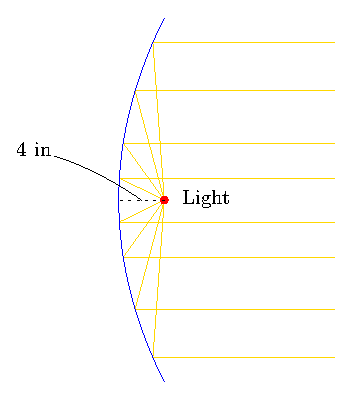
\includegraphics{./carlight}
\vspace{10in}
\end{frame}

\begin{frame}[label={sec:orgfa745e0}]{Example}
\end{frame}

\begin{frame}[label={sec:orgadf6ffa}]{Example}
A satellite dish is shaped like a paraboloid of revolution. This means
that it can be formed by rotating a parabola around its axis of
symmetry. The receiver is to be located at the focus. If the dish is
12 feet across at its opening and 4 feet deep at its center, where
should the receiver be placed?

\vspace{10in}
\end{frame}

\begin{frame}[label={sec:org1eace95}]{Example}
\end{frame}

\begin{frame}[label={sec:org9540abf}]{Example}
One more application of parabolas is projectile motion.  If we throw
an object straight into the air with an initial velocity of \(v_0\)
feet per second and from a height of \(h\) feet above ground level, it
can be shown using physics that the equation that tells you the height
of the object (in feet) after \(t\) seconds is

\[s(t) = -16t^2 + v_0 t + h\]
\vspace{10in}
\end{frame}

\begin{frame}[label={sec:org9ef9710}]{Example}
You throw a ball straight into the air (from the ground) with an
initial velocity of 80 feet per second.  What is the maximum height
that the ball attains?

\vspace{10in}
\end{frame}

\begin{frame}[label={sec:orgb42ed82}]{Example}
\end{frame}
\end{document}